% Paper A: corpus + measure. Assembled by ../assemble.py; hand-written
% files: abstract, intro, record_head, owner_links, validation_head,
% hazard_head, access. gen_*.tex are generated from ../../v3_rp and ../../v3.
\input{../../v3_rp/preamble}
\newcommand{\onlineappendixnote}{\url{https://aporia.institute/tm-vocabulary/online-appendix/themes_T50.html}}
\graphicspath{{../../}}
\makeatletter\def\input@path{{./}{../../}{../../v3_rp/}}\makeatother
\title{\bfseries An Event-Dated Corpus of US Trademark Prosecution\\
\large and a Two-Sided Measure of Vocabulary Position}
\author{Eric Silver\thanks{Independent researcher; formerly a PhD candidate
at Carnegie Mellon University.}}
\date{Draft, September 2026 --- Paper A of two}

\begin{document}
\maketitle
\begin{abstract}
\noindent The USPTO publishes every US trademark application filed since
1884, together with the history of what happened to it. We re-parse all
13.99 million of these case files into 242 million dated events, so that
every mark can be followed step by step from filing through examination,
registration, the sworn five-year proof of continued use, and the
year-ten renewal, with counsel of record, filing basis and owner domicile
read from the record, and owners linked by name to SEC reporting,
Form~D fundraising rounds and patent assignees. The dates matter because
the USPTO's terminal status codes run the maintenance deadlines together:
a registration cancelled for missing the year-six proof of use and one
cancelled at the year-ten renewal share a code. Once each cancellation is
dated, the record shows which deadline a lapsed mark failed, and the
five-year proof becomes something the literature has not had: a dated,
product-level record of whether the goods behind a registered mark were
still being sold. On this corpus we build a measure of where a filing's
language sits relative to its industry. A topic model reduces each
goods/services description to a mix of themes---an online offering, say,
or an artificial-intelligence application---and we compare that mix, by
Kullback--Leibler divergence, with what the filing's own Nice class filed
in the five years before its date and in the five years after. The
average of the two comparisons is the filing's \emph{atypicality}: how
unusual its language is for its industry. Their difference is its
\emph{lead}: whether its language ran ahead of or behind where the
industry's language was moving. We validate the measure by rescoring
identical filings under three partitions of the vocabulary, two reference
weightings, five window constructions, a second model seed, and with the
pervasive verbatim text duplication removed. Lead survives every
variation and predicts cancellation for non-use at the five-year proof
($+2.3$, $+2.6$ and $+1.9$ points under the three partitions; $+1.4$ with
design controls, $t = 8.3$). Atypicality does not: its apparent effects
belong to the partition or to a control. We document two hazards for
trademark-text research---scoring words rather than themes measures
description length ($r = -0.68$ with log distinct terms), and firm-level
correlations built on word scoring dissolve or reverse under theme
scoring on identical samples. Within firm, the measure is orthogonal to
patenting. The corpus, the scores, the code, and an interactive per-class
appendix are public.

\medskip
\noindent\emph{Keywords:} trademarks; administrative data; text as data;
topic models; Kullback--Leibler divergence; innovation indicators.\\
\emph{JEL:} C81, O34, O31, L10.
\end{abstract}

\section{Introduction}\label{sec:intro}

A US trademark application carries a description of the goods or services
the mark will cover. It is written to secure scope of protection, it is
dated, it is public, and it is filed by the millions of firms that never
patent. The literature that reads trademarks as innovation data has used
the filing's count, its class, its breadth and its renewal
\citep{Castaldi2020, Flikkema2019, Dinlersoz2018}; the description itself
has entered only piecemeal, as breadth counts or similarity scores. This
paper builds two research assets on the description and on the
prosecution record that surrounds it, states what each can and cannot
support, and makes both public.

The first asset is a corpus. The USPTO publishes every application since
1884 with its prosecution history, and terminal status codes are what the
literature has read from it. Status codes conflate events that the
maintenance schedule keeps apart: a registration cancelled for failing the
year-six proof of continued use and one cancelled at the year-ten renewal
share a code. Re-parsing all 13.99 million case files into 242 million
dated events assigns each cancellation to the proof it failed by its date,
and records for each filing the office actions, the responses and their
latency, counsel of record, the statutory filing basis, and the owner's
domicile. The five-year proof of continued use thereby becomes a dated,
sworn, product-level survival record available for every registered mark
more than seven years old. Owners are linked by normalized name to SEC
reporting, to Regulation~D rounds, and to PatentsView patent assignees.

The second asset is a measure. Each description is reduced to themes by a
topic model fitted once over the whole corpus, and its theme mix is
compared, by Kullback--Leibler divergence, to what its own Nice class
filed in the five years before and the five years after its date. The
average of the two divergences is the filing's \emph{atypicality}, how
unusual its language is for its industry; their difference is its
\emph{lead}, whether its language sat ahead of or behind where the
industry's language was moving. The two-sided reference is what separates
\emph{unusual} from \emph{early}, and the two components predict
different things.

The measure is validated by variation rather than by a single fit. The
identical filings are rescored under three partitions of the vocabulary
(fifty global themes, five hundred, fifty fitted per class), two
reference weightings, five window constructions, a second model seed at
fixed resolution, and with and without the 47\% of registrations whose
text is shared verbatim with another filing. Lead survives every
variation and predicts failure at the five-year proof: $+2.3$, $+2.6$ and
$+1.9$ points from the most lagging to the most leading fifth under the
three partitions, $+1.4$ points with class-by-cohort fixed effects,
drafting and filer controls and owner-clustered errors ($t = 8.3$).
Atypicality does not: its protective effect at the proof falls from $4.4$
points under global themes to $0.7$ under per-class themes, because a
global model reads a theme imported from another class as atypical, and
its sign at the SEC-reporting margin depends on how description length is
held.

Two hazards follow for any research that scores trademark text, and both
are documented on identical samples. Scoring words rather than theme
distributions measures description length: the divergence decomposes into
a surprise term and a spread term, the spread term is bounded by the
filing's distinct-term count, and term-scored atypicality correlates with
log distinct terms at $-0.68$. Firm-level correlations built on word
scoring, which are the kind the literature reports, dissolve or reverse
under theme scoring on the same firms; the signal they carry is unsigned
lexical specificity, not vocabulary position. A third caution concerns
the sample rather than the score: applicants who refile an abandoned
application rewrite toward their class's typical language from both
tails, so every registered description is in part a conformed one, and
pooling granted with abandoned filings mixes the examiner's selection
with the market's.

What the measure predicts about pioneering, about industry waves, and
about which firms reach the capital markets is the subject of a companion
paper; here those outcomes appear only as validation, and the paper makes
no claim about mechanism. Section~\ref{sec:record} describes the corpus,
the steps of the record and the three outcomes it dates.
Section~\ref{sec:measure} builds the measure and shows, on named filings,
what themes resolve and what they miss. Section~\ref{sec:related} settles
nomenclature against the innovation literature's existing terms.
Section~\ref{sec:validation} tests the measure against registration, the
five-year proof, patenting and SEC reporting. Section~\ref{sec:robust}
reports what changes under every alternative construction tried.
Section~\ref{sec:practices} states the practices that follow for
trademark-text research, and Section~\ref{sec:access} describes the
public artifacts.

\section{The record: from case files to dated events}\label{sec:record}

\subsection{Corpus and parse}

The USPTO Trademark Annual Applications backfile (product TRTYRAP) is the
complete record of US trademark filings from 1884 onward: 13.99 million
case files, each carrying the goods/services description by class, the
prosecution history, and the ownership and correspondence records. The
prosecution history is a list of coded events with dates. This paper
re-parses every case file into 242 million dated events, keyed by serial
number, so that for each application the sequence of office actions,
responses, allowances, statements of use, registration, Section~8 and
Section~9 filings, cancellations and renewals is available with its
date.\footnote{Event codes are read against the USPTO's own event-code
dictionary. Terminal status codes are retained for cross-checking: 700
registered; 701--705 Section~8 accepted; 710 cancelled for Section~8
failure; 800 renewed; 900 expired. The year-six cancellation and the
year-ten cancellation share status 710 and are separable only by event
date, which is the reason the corpus is event-dated.} From the same files
the parse reads counsel of record on each filing (and, for refilings, on
each attempt separately), the statutory filing basis (use, intent to use,
\S44(e) home registration, \S66(a) Madrid extension), the owner's
domicile, and the owner name, which is normalized --- uppercased,
stripped of punctuation and of two dozen legal suffixes --- so that
\textsc{acme corp.} and \textsc{acme corporation} are one owner.
\citet{Graham2013} describe the administrative data; the event-dated
parse adds the full prosecution timeline of each case.

Response latency in prosecution is a by-product of the parse and is
retained as a health indicator: the median days from an office action to
the applicant's response, per filing.

\subsection{The steps, the samples, and the conventions}\label{sec:gates}

The record's steps, the outcome names, and the counting conventions are
set out once, here, and every later section uses them.

A US trademark passes through a sequence of dated, high-stakes steps, and
each step leaves a record. An application is filed with a goods/services
description; an examiner reviews it, often issuing office actions the
applicant must answer; if allowed and (for intent-to-use filings) a sworn
statement of use is filed --- the proof that the mark has entered commerce
--- the mark registers. Registration starts a maintenance clock: in years
five to six the owner must file a Section~8 declaration proving continued
use in commerce, with a six-month grace period --- the \emph{five-year
proof of continued use}, the paper's central outcome; around year ten a
combined Section~8 declaration and Section~9 renewal is due, and every ten
years thereafter. A mark that misses a proof is cancelled. Madrid Protocol
registrations (\S66(a) basis) file Section~71 declarations on the same
schedule and are flagged separately throughout. \citet{Graham2013}
describe the administrative data; the event-dated corpus built here adds
the full prosecution history of each case, so a cancellation is assigned
to a specific proof by its date rather than inferred from a status
snapshot.\footnote{Cross-checked against the USPTO status-code dictionary:
700 registered; 701--705 Section~8 accepted; 710 cancelled for Section~8
failure; 800 renewed; 900 expired.}

\begin{table}[h]\centering\small
\caption{The trademark funnel in this corpus. Registration counts are
unique serials; five-year-proof outcomes are event-dated (a Section~8
cancellation at registration age 4.0--8.5 years). Source: the re-parsed
USPTO application backfile, scored as in this section.}
\label{tab:funnel}
\begin{tabular}{lrr}
\toprule
Stage & $n$ & Share \\
\midrule
Debut filings scored, 1995--2018 (owners' first filings) & 3{,}589{,}068 & \\
\quad reached registration & 2{,}066{,}600 & 57.6\% \\
\midrule
All unregistered class-records filed 1995--2018 & 3{,}798{,}318 & \\
\quad never filed statement of use & & 42.6\% \\
\quad stopped responding in prosecution & & 45.3\% \\
\quad removed adversarially & & 4.3\% \\
\midrule
Registrations 2002--2018, scored, unique serials & 3{,}104{,}534 & \\
\quad failed the five-year proof of continued use (event-dated) & & 52.3\% \\
\midrule
Passed the five-year proof, cohorts 2002--2013, status known & 1{,}129{,}724 & \\
\quad failed at the year-ten renewal & & 39.1\% \\
\bottomrule
\end{tabular}
\end{table}

Three named outcomes recur (Table~\ref{tab:funnel}). \emph{Failing to
register}: the application never completed, which happens by the
applicant's own inaction in roughly nine cases of ten
(Section~\ref{sec:val_registration}). \emph{Failing the five-year proof of
continued use}: a registration cancelled for non-use at registration age
4.0 to 8.5 years, which means the product the mark named left commerce
within six years (Section~\ref{sec:val_gate}).
\emph{Reaching the SEC record}: the owner appears in dated SEC events ---
a priced Form~D round, financial reporting, a listing
(Section~\ref{sec:links}).

Outcomes are rates, so every estimate is a shift in a probability and is
stated in percentage points against the base rate it shifts: $+1.4$pp on
a 52.3\% base means 53.7\% against 52.3\%. The basic comparison is the
outcome rate of the fifth of filings with the highest lead minus that of
the fifth with the lowest, with the fifths cut inside a single Nice class
and year so that no difference between industries or between years
enters; regression tables add drafting and filer controls and cluster
errors on the owner. Where a continuous version is given, it is the
change in the outcome for a one-standard-deviation change in the axis, in
percentage points.

Counting differs by table. A filing may claim several Nice classes at
once, so a \emph{class-record} counts it once per class while a
\emph{registration} counts it once by serial number; a \emph{debut
filing} is an owner's first, one per owner. A \emph{cohort} is the set of
registrations issued in a calendar year; where a split is instead by
filing year, the text says so.

Two windows bound the samples, each set by an institutional fact. Scoring
runs 1995--2019: a full five-year past reference does not exist before
1990 and a full forward reference does not exist after 2020, and the 1995
cut is about two years more conservative than the measured burn-in
requires (Section~\ref{sec:burnin}). Five-year-proof cohorts run
2002--2018: cancellations post at about registration age six and a half,
the record ends in April 2026, so 2018 is the last cohort whose window
has essentially elapsed, and 2002 is the conventional lower cut for this
corpus --- a bound that matters, because carried back to the first
scoreable cohorts the lead penalty was larger than it has ever been
since, as the companion paper shows.

% Neighbours/nomenclature moved to Section 2 (rp_related) for the RP build.

\subsection{Self-filed and professionally filed applications}\label{sec:representation}

Counsel of record is observed on every filing. Represented applications
are 73\% of filings over 1995--2018, falling from 85\% in 1995 to 68\% in
2018 as online self-filing spread. The two populations file differently
and fare differently:

\begin{center}\small
\begin{tabular}{lrrr}
\toprule
 & Share of filings & Reached registration & Median terms (009 / 035) \\
\midrule
Represented & 73.3\% & 61.9\% & 28 / 26 \\
Self-filed  & 26.7\% & 45.6\% & 21 / 17 \\
\bottomrule
\end{tabular}
\end{center}

\noindent Self-filers write shorter descriptions (a median of 21 terms
against 28 in the software class, 17 against 26 in advertising and
retail), sit closer to their class's usual language, and lean slightly
further ahead of it. Because who drafts affects both the language and
the outcome at once, the five-year-proof regressions control for counsel
of record and report their estimates separately for the two groups.
Figure~\ref{fig:sankey} draws the full flow from filing to registration
split by drafter.


\subsection{Office actions and refiling: applicants rewrite toward the class}\label{sec:amend}

An application that is abandoned is usually the end of that attempt: among
2.28 million abandoned applications, 3.6\% are followed within six years
by the same owner filing the same mark again in the same class, and 1.5\%
by one that then registers. The refilings that do occur show what an
applicant changes. Of the 42{,}115 abandoned applications whose owner
later registered the same mark in the same class, 74\% carry a different
goods/services description the second time. To see which way the text
moved, we score each of these registrations twice: once on the text of
the abandoned first attempt, once on the text it registered with. Both self-filers and represented owners
rewrite toward the class's typical description: originals in the most
atypical fifth lose $0.39$ nats of atypicality, and originals in the most
conventional fifth gain $0.16$. Refilings that reuse the identical text
move by less than $0.01$ at every position, so the convergence is in the
writing. Who drafts changes the extent but not the direction: owners who
hire counsel for the second attempt rewrite most often (82\%) and their
descriptions lengthen by 16\%; counsel rewriting their own earlier draft
rewrite least often (72\%) and shorten by 4\% (Figure~\ref{fig:refile}).
Lead barely moves once we account for the reference windows themselves
shifting with the later filing date.



Figure~\ref{fig:refile} shows the goods/services description before and
after a rewrite, for the 31{,}084 refilings in Section~\ref{sec:amend}
whose text changed. A pair is an abandoned application and the same owner's
later registration of the identical mark in the same Nice class within six
years; the earliest registered refiling is kept. Counsel of record is read
from the prosecution history of each filing separately, so a pair can change
representation between attempts. Atypicality is on the production scoring;
length is the word count of the normalized description.

\begin{figure}[!htbp]\centering
\includegraphics[width=\textwidth]{results/refile_prepost.png}
\caption{Rewritten refilings: mean atypicality and mean description length
of the abandoned filing (grey) and of the registered refiling (red), by
representation on the refiling and by the change in representation between
the two attempts. Mean atypicality falls by $0.01$ to $0.03$ nats in every
group except counsel-then-self, where it is unchanged. Length rises by six
words where counsel is hired for the
second attempt and falls by one where counsel rewrites counsel.}
\label{fig:refile}
\end{figure}

The means understate the convergence, because it runs in both directions.
By fifth of the original's atypicality, the change is $+0.16$, $+0.14$,
$+0.06$, $-0.06$ and $-0.39$ nats from the most conventional fifth to the
most atypical, and within a point of that profile in each of the four
representation groups. Identical-text refilings change by $+0.002$ to
$+0.008$ across the same fifths. On lead, the changed-text profile runs
$+0.046$ to $-0.072$ and the identical-text profile $+0.014$ to $-0.054$;
the difference is the rewriting, the rest is the reference windows moving
with the later filing date.


\subsection{Owner links: SEC reporting, Regulation~D rounds, patents}\label{sec:links}

Owners are matched to three external records by normalized exact name.
\emph{SEC reporting} is any appearance of the owner as a registrant in the
Commission's EDGAR filer index; roughly half the matched firms carry a
ticker and the rest report for other reasons, and the two halves are
distinguished by the Commission's company-ticker file. \emph{Regulation~D}
rounds are Form~D notices of exempt offerings, electronic and therefore
complete only from 16 March 2009, so any analysis of a funding ladder is
built on debuts from 2009. \emph{Patents} are PatentsView assignee records
\citep{PatentsView}, matched on the same normalized name.

The SEC match runs over a candidate universe of all 5.67 million owners in
the corpus; names resolving to more than one registrant are dropped rather
than assigned, and one match is kept per owner string. That yields
19{,}889 matched owners covering 7{,}588 registrants. Validation on 22
companies that indisputably went public --- across software,
pharmaceuticals, food, apparel, aerospace and autos --- matches all 22; a
random sample of 25 matches carrying at least three filings was inspected
by hand and none was wrong, which is a check on gross failure modes rather
than a precision estimate. The linkage is nonetheless a name match, and
that bounds what can be read from it: firms with distinctive names are
easier to match than firms with generic ones, and distinctiveness of a
name plausibly travels with distinctiveness of the goods/services text.
Section~\ref{sec:validation} returns to which results survive that bound.

\section{The measure}\label{sec:measure}\label{sec:construct}

\subsection{Two readers, one living backwards}

Imagine two readers of a filing's goods/services description, each having seen
a disjoint half of its industry. One has read only what the industry filed in
the five years before it. The other, living backwards as Merlin was said to,
has read only the five years after. Each is asked how surprising the wording
is. The measurement is how much they disagree: a description that startles the
first reader and not the second arrived before its industry's language moved
that way.

Both windows are anchored on the filing's own date, spanning the 1,826
days before it
and the 1,826 days after; both exclude the filing date itself, so a filing
never appears in the reference of another filing made the same day, and no
two filings made on different days share a reference. Inside a window every day counts the same. The measure asks whether
wording is unusual against a period, not whether it is ahead of a trend
inside that period; it has no momentum channel.

\subsection{What is measured}

The quantity is information content in Shannon's sense. Something that
happens with probability $p$ carries $\log(1/p)$ of information when it
happens: a common thing carries little, a rare thing a lot. Here the things
are the themes a description draws on, and the probabilities are how often
the filing's own industry drew on each of them in the reference window. A
filing's score asks, in effect: how surprising is this mix of themes to
someone who has only seen what the industry files? Formally it is the
average information content of the filing's themes under its industry's
frequencies, weighted by how heavily the filing uses each, less the same
average taken under the filing's own frequencies.

The apparatus is that of \citet{Murdock2017}, developed on Darwin's reading
notebooks, and \citet{Barron2018}, who extended it to French Revolution
parliamentary debates. They score a document against those before it and
again against those after, calling the two quantities \emph{novelty} and
\emph{transience} and their signed difference \emph{resonance}. Their object
was the life of ideas: how often an idea appeared, and how ideas stood in
relation to one another, across one reading life or one assembly's debate.
The object here is the composition of commercial offerings, which components
a product or service is described as having, and how that composition shifts
across an industry over time. The arithmetic carries over unchanged. The
interpretation does not: their document has one author and the reference
stream is that author's own reading, so a high value says something about a
mind; here a filing is scored against other firms' filings, and its author is
usually counsel drafting for scope of protection. The same shift renames
what the model finds. In those settings, and in the name of the method,
latent Dirichlet allocation identifies \emph{topics} --- what a document
is about. A goods/services description is not about anything in that
sense; it lists components, and across millions of filers a cluster of
terms that co-occur (\emph{video, music, games, electronic, audio}) is a
component many offerings share --- a theme the entrants' offerings
evidence, not a subject. \emph{Theme} is the word used throughout;
\emph{topic} appears only in the model's name.

\subsection{From a description to two numbers}\label{sec:definitions}

\paragraph{Counting words.} A description is reduced to a bag of words: the
text is lowercased, split into tokens of three or more letters, and counted,
with adjacent pairs counted as tokens in their own right so that
\emph{computer software} registers alongside \emph{computer} and
\emph{software}. Order is discarded. Take the filing for \textsc{Amazon.com},
lodged in the advertising and retail class on 18 April 1997:

\begin{quote}\small
computerized on line search and ordering service featuring the wholesale and
retail distribution of books, music, motion pictures, multimedia products and
computer software in the form of printed books, audiocassettes,
videocassettes, compact disks, floppy disks, CD ROMs, and direct digital
transmission
\end{quote}

\noindent Of its 45 distinct terms, 36 are in the theme model's vocabulary,
among them \emph{computerized}, \emph{search}, \emph{ordering},
\emph{ordering service}, \emph{retail}, \emph{distribution}, \emph{printed
books} and \emph{digital transmission}.

\paragraph{Grouping words into themes.} Each filing is then re-described
in a fixed, much smaller set of coordinates. We run latent Dirichlet
allocation once over a stratified sample of the whole corpus, all 45
classes together. The model develops a list of 50 themes --- clusters of
words that tend to occur together --- and infers, for any filing, to what
degree its description invokes each one. Nothing supervises this; the
clusters come from co-occurrence alone, and a theme is read off from its
leading words: one collects the vocabulary of media and entertainment
goods, another retail store services, another downloadable and online
software. Re-described this way, a filing becomes a mix of themes, and
two kinds of question open up: how a theme fares over time within a class
--- how much of the class's language an online-offering theme accounts
for, year by year --- and how the filings that invoke it fare. This
build --- fifty global themes, per-filing five-year windows, flat
weighting --- is the production scoring, used for every estimate unless
the text states another. The themes are shared across classes; what is
specific to a class is the reference: the average theme proportions of
that class's own filings in the window. The Amazon filing draws on six
themes at more than a twentieth of its weight: $0.41$ on media and
entertainment goods (\emph{video, computer, electronic, music, games,
audio}), $0.15$ on computer and information services (\emph{services,
computer, software, information, data}), $0.13$ on retail store services
(\emph{store, retail, store services, featuring}), $0.10$ on printed matter
(\emph{paper, books, printed, cards, stationery}), $0.09$ on downloadable and
online software, and $0.07$ on marketing of consumer goods. The online
appendix lists every theme with its leading words and its weight in each
class.\footnote{\onlineappendixnote}

Fifty is coarse, roughly one theme per industry.
Section~\ref{sec:three_scorings} refits the model at 500 themes and
separately at 50 themes within each class and repeats the five-year-proof
analysis under each; Section~\ref{sec:robust} reports the resolution sweep
and a second fit at the same resolution with a different seed. Fifty is
kept elsewhere because it is the coarsest resolution at which every result
holds, and because its software-class lead contrast sits at the low end of
the resolutions tried (only the 100-theme refit returns less).

\paragraph{Comparing against the two references.} Write $P$ for the filing's
distribution over themes, and $Q^{-}$ and $Q^{+}$
for that distribution averaged over every same-class filing in the two
windows, $[d_i - W,\, d_i)$ and $(d_i,\, d_i + W]$, with $W = 1{,}826$ days.
How far $P$ sits from a reference $Q$ is the Kullback--Leibler divergence,
\[
  \mathrm{KL}(P \,\|\, Q) \;=\; \sum_{k} P_k \log \frac{P_k}{Q_k},
\]
a sum over the 50 themes, zero when the two distributions agree and growing as
the filing puts weight where the industry puts little. It is measured in nats,
the natural-log unit. Write
\[
  K^{-} = \mathrm{KL}(P \,\|\, Q^{-}),
  \qquad
  K^{+} = \mathrm{KL}(P \,\|\, Q^{+}),
\]
so $K^{-}$ is what the first reader feels and $K^{+}$ the second: the
filing's past-facing and future-facing surprise.

\paragraph{Taking the difference.} Amazon's filing is scored against 41{,}166
earlier filings and 146{,}532 later ones, giving $K^{-} = 1.286$ and
$K^{+} = 1.163$. The two axes used throughout are their average and their
signed difference:
\[
  \underbrace{A \;=\; \tfrac{1}{2}\left(K^{-} + K^{+}\right)}_{\text{atypicality}},
  \qquad
  \underbrace{L \;=\; K^{-} - K^{+}}_{\text{lead}} .
\]
For Amazon, $A = 1.225$ and $L = +0.123$: against its own class, its
atypicality is at the 47th percentile and its lead at the 94th. The
industry moved toward this description in the five years after it was filed
and had not been writing that way in the five years before.
Table~\ref{tab:nomenclature} maps the terms and their nearest occupants
in the literature; the signed difference is written $L$ throughout and
its magnitude $|L|$.

What ``early'' means is visible in the themes themselves: the three themes
that carry most of Amazon's description --- retail store services, media
and entertainment goods, and the still-small online-software theme --- all
became more common in class 035 over the following five years, the last
nearly doubling, while the two minor themes it touched receded. The filing
is closer to the class's future composition than to its past one; the
supplementary material tabulates the six theme shares.

Why the average and the difference, rather than the two surprises
themselves? Because $K^{-}$ and $K^{+}$ correlate at $0.988$ on the
software class: a filing far from its class's past is almost always far
from its future too, so entering both is close to entering one variable
twice. The average collects that large shared component --- how far from
the class the filing sits --- and the difference collects the small
residual that carries the timing. Nothing more than a sum and a
difference is taken, with no weights estimated, and the two resulting
regressors are nearly uncorrelated ($+0.036$ against each other, where
$K^{-}$ alone would give $+0.114$). The cost is that $L$ is a small residual of
two large quantities, about a sixth of either level's spread, which
Section~\ref{sec:robust} quantifies.


\paragraph{Why the words are not scored directly.} The themes are an extra
step, and the words themselves could be compared to the reference: build the
filing's distribution over the class vocabulary from the words it uses, do
the same for every filing in the window, and take the divergence. The paper
reports that scoring as a cross-check. It cannot be the primary one, because
a divergence measured on words mostly counts the length of the filing. The
divergence is an average surprise less a spread: for any two distributions,
\[
  \mathrm{KL}(P \,\|\, Q) \;=\; \underbrace{-\textstyle\sum_k P_k \log Q_k}_{\text{how unexpected these words are}}
  \;-\; \underbrace{\left(-\textstyle\sum_k P_k \log P_k\right)}_{\text{how spread out the filing is}} ,
\]
and the spread of a filing over words is bounded by how many distinct words it
has: a description using $k$ terms cannot spread over more than $k$ of them,
so its spread cannot exceed $\log k$, while the reference is spread over about
900 terms. A five-word description is charged the whole difference in width,
roughly five nats, before any of its content is considered. To show this
directly, we took 3{,}000 software-class filings of at least 150 words,
scored each against one fixed reference, then cut each down to a random
handful of words and rescored it. Across a fiftyfold cut in length, the
surprise term moves by $0.016$ nats while the spread term moves by
$2.9$: essentially all of the change in the score is the length, not the
content. Synthetic filings drawn at random from the reference itself
track $\log(\text{distinct terms})$ to within a fiftieth of a nat
(supplementary material). Term-scored atypicality correlates with
the log of a filing's distinct term count at $-0.68$ in the software
class.

Themes break the coupling because the 50 coordinates are always occupied.
Under term scoring the effective number of coordinates a filing spreads over
rises seventeenfold from the shortest descriptions to the longest; under
themes it varies by less than a third, and not monotonically: a three-word
fragment gives the model little evidence, so its inferred proportions stay
close to the prior and spread across many themes. The spread term no longer
tracks length, and the score is dominated by the surprise term.
Theme-scored atypicality correlates with the log term count at $-0.22$ in
the software class and $-0.10$ in advertising and retail, against $-0.68$
and $-0.62$ under terms.

\paragraph{What the themes see, and what they do not.} The score compares a
filing's theme proportions to the average proportions of its industry, so it
reads which themes a filing draws on and how heavily. It does not, in any
material way, read how a filing combines them. To check this, we took
each filing's two leading themes on a 150{,}000-filing software-class
sample and asked how often that pair occurs together, relative to how
often the two themes occur separately. How rare the themes are
individually explains 70\% of the variance in atypicality; how unusual
the pairing is adds under two points on top of it. A filing assembled from ordinary parts in a
genuinely new configuration is therefore close to invisible to this measure.

Combinations can be scored in their own right, at two levels
(construction detail in the supplementary material). The first is
\emph{pair lead}: whether the class later moved toward the filing's
arrangements of themes. In the software class it is penalised much as
lead is ($+2.3$ points at the five-year proof, $t = 8.4$, while
correlating with lead at only $-0.16$). But it does not generalize.
Corpus-wide it is zero raw and $+0.5$pp net of lead and atypicality
(owner-clustered $t = 4.2$), significantly positive in 13 of 43 classes
and significantly negative in 3 --- including $-2.1$ in advertising and
retail --- so we report it as a class-specific bound rather than a second
construct. The second is word-level \emph{recombination}: adjacent word
pairs that are new to the class while both words are established there,
novelty assembled from familiar components
\citep{Fleming2001, Uzzi2013}. In the same class it is rewarded: the top
fifth fails $2.8$ points less with lead and atypicality held
($t = -10.4$), and it is uncorrelated with pair lead ($r = -0.01$). The
construct sees neither arrangement channel, and where they act they run
in opposite directions, so its blindness to combination is a bounded
omission rather than a hidden bias in one direction.

\subsection{Within class, not across it}

Goods/services descriptions are drafted to secure scope of protection, not to
describe a product distinctively, and counsel reuse language from the USPTO's
own Acceptable Identification of Goods and Services Manual, from house
precedent, and from competitors' successful filings. Identical wording across
unrelated firms is therefore common, and it carries through to the scores:
17\% of scored registrations issued 2002--2018 share a value with another
filing in the same class and registration year. Within a class, the measure picks up departure from a shared
drafting convention. Across classes it does not: a class where the Manual
supplies dense standard language shows a compressed distribution of
atypicality, and one where firms describe novel services in prose a wide one,
for reasons unrelated to how innovative either industry is. Every estimate is
therefore taken within class and year, and magnitudes compare across classes
only as signs and orderings.

The vocabulary is positional rather than causal: a leading filing was
ahead of its industry's language, which implies a trajectory without
asserting the filing caused it.

\subsection{Term scoring measures length; theme scoring does not}\label{app:representation}

Figure~\ref{fig:representation} puts the two representations side by side
over the same axes, with each hexagon coloured by the mean length of the
filings in it. Under term scoring the colour runs from dark near the
origin --- a median of about 200 terms --- to near-white at the far end,
where the median is eight. That gradient is the measurement problem: a
filing scores as atypical largely because it is short. Under theme scoring
the same surface is a narrow band of roughly uniform tone.

Two filings are marked in both columns. Under the production scoring they
behave differently from one another, which is the point. \textsc{Amazon.com}
(1997) is at the 98th percentile of lead on terms and the 94th on themes,
but only the 40th and 47th
percentiles of atypicality, so both agree that it was early and neither
mistakes it for strange. Apple's \textsc{iPod} (2001) divides them: the 31st
percentile of lead on terms against the 62nd on themes. The surfaces plotted
here are on the class-year build the figure was generated from, where the
length gradient is starkest; the percentiles just quoted are on the per-filing
build used for every estimate.

\begin{figure}[!htbp]\centering
\includegraphics[width=\textwidth]{results/representation_appendix.png}
\caption{Mean filing length across the two axes, by representation and
class, for filings 1995--2019 scored on per-filing reference windows. The
horizontal axis is surprise against the preceding five years, the vertical
axis surprise against the following five; a filing on the dashed diagonal
is equally far from both, and distance below it is lead. Hexagons holding fewer than 25 filings are blank; the retained
hexagons cover over 99.4\% of filings in every panel. The colour scale is
shared across panels; the axis ranges are not, because term-scored and
theme-scored KL are not on a common scale, so only shape and colour
gradient are comparable across columns. Both
columns are drawn on the filings the per-filing windows score, which
differ between representations by under one percent.}
\label{fig:representation}
\end{figure}

Each representation has the virtue the other lacks: theme scoring is
independent of document length, which term scoring is not, while term
scoring resolves novel word \emph{combinations}, which theme scoring does
not. We therefore use theme scoring for every estimate, because the
length confound contaminates firm-level comparisons, and term scoring for
every worked example, because the theme basis has no coordinate for the
language the examples turn on.

\subsection{How three filings encode}\label{app:exhibit}

Table~\ref{tab:exhibit} traces three filings through term scoring and theme
scoring at $T \in \{50, 200, 500\}$ --- three kinds of novelty, and how each
representation handles them.

\textsc{Amazon.com} (1997, advertising/retail) is \emph{combinatorial}
novelty: every word is ordinary, but the bigrams assemble an invention
(``computerized line,'' ``line search,'' ``search ordering''; class
document frequencies 379, 134, 355). The filing's text reads ``on line''
as two words, the standard spelling in 1997, before \emph{online}
lexicalized into a single token; the analyzer drops the stopword ``on''
and the bigram ``line search'' survives
stopword removal. The novelty was necessarily combinatorial
because the word for it did not yet exist. Term scoring sees these
bigrams; under theme scoring at every resolution all of them are out of
vocabulary and the filing reads as a media retailer that uses computers.

\textsc{Kombucha} (1997, beer/soft drinks) is \emph{lexical} novelty: the
new thing arrives as new words (\emph{kombucha} df 567, \emph{saccharose}
out of vocabulary even at the class level). The word \emph{kombucha} is in
the theme vocabulary but, with no kombucha-like theme, the filing loads on
a generic beverages theme at every $T$ (Table~\ref{tab:exhibit}).

\textsc{Ethereum} (2018, software) is \emph{wave} novelty: emergent
vocabulary already diffusing (\emph{blockchains}, \emph{distributed
computing}). It loads on generic software and services themes at every
resolution, including $T = 200$, which does contain a
cryptocurrency/blockchain theme; there, the eleven occurrences of
\emph{software} dominate the theme assignment.

\begin{table}[!htbp]\centering\small
\caption{Top theme loading for three filings, by representation. Term
scoring resolves the novel content of all three; theme scoring resolves
none of it at any tested resolution.}
\label{tab:exhibit}
\begin{tabular}{lp{3.1cm}p{3.1cm}p{3.1cm}}
\toprule
& \textsc{Amazon.com} & \textsc{Kombucha} & \textsc{Ethereum} \\
& (1997) & (1997) & (2018) \\
\midrule
novel content (term) & line search, search ordering & kombucha, saccharose & blockchains, distributed computing \\
$T=50$ & video, computer, music (0.40) & beverages, fruit, drinks (0.64) & software, online, downloadable (0.33) \\
$T=200$ & entertainment, video, games (0.29) & beverages, drinks, coffee (0.60) & field, services, development (0.37) \\
$T=500$ & computer, software, data (0.22) & beverages, drinks, fruit (0.61) & software, online, computer (0.49) \\
\bottomrule
\end{tabular}
\end{table}

The pattern across the row is the measurement point in miniature: theme
scoring cannot represent combinatorial novelty (Amazon), dilutes lexical
novelty (Kombucha), and majority-votes away wave novelty (Ethereum) even
when a fitting theme exists. That the mark-level outcome results are
nearly identical under both scorings despite this blindness is what
licenses theme scoring as a robustness instrument; that the firm-level
results diverge is what exposes them as artifacts of the lexical
specificity term scoring additionally captures
(Section~\ref{sec:robust_hazard}).

\subsection{Scores are interpretable from 1995}\label{sec:burnin}

\emph{Burn-in} is the span at each end of the corpus where the reference
windows cannot be filled, so scores there reflect a thin reference rather
than the text being scored.

The signal depends on having enough past and future filings to populate
the references. The 5-year past window is incomplete before 1990 and the
future window after 2020, and both zones are excluded
(Figure~\ref{fig:burnin}). The burn-in cut is set empirically. A thin
past reference inflates past-facing surprise, and profiling that bias
across all 44 sufficient-volume classes gives a median absolute bias of
$\sim$2.0 nats in 1990, 0.25 in 1991, 0.10 in 1992, and 0.04 from 1993
onward --- below any effect size interpreted in this paper. The
1995--1997 deviations ($\sim$0.15--0.17) are not burn-in: mechanical
contamination declines monotonically as the windows fill and cannot
rebound, so these reflect a genuine vocabulary shift in the corpus
during the dot-com period. Estimating a separate burn-in length per
class turns out to track each class's noise floor rather than its
reference density, so a single standard cut at 1995 is used,
conservative by about two years.

\begin{figure}[!htbp]\centering
\includegraphics[width=0.85\textwidth]{results/burnin.png}
\caption{Reference-window density by year on log scale. Hatched regions
are the past-side and future-side burn-in zones where the 5-year window is
incomplete. The dotted line marks the 1995 analysis cut. The windows
decide the score at the filing date; the gate outcome is read separately,
at registration age six to seven.}
\label{fig:burnin}
\end{figure}


\section{Neighbours and nomenclature}\label{sec:related}

\subsection{Trademarks as innovation data}

A trademark filing is a dated, costly, public disclosure made by the
millions of firms that never patent, and a literature has grown around
reading it as an innovation indicator \citep{Castaldi2020, Willeke2026}.
Trademark counts and breadth predict venture valuations
\citep{Block2014}; filing timing tracks innovation processes
\citep{Seip2018}; and trademarks mark the product-market side of
innovation that patents miss \citep{Flikkema2019, Flikkema2025}.
Census-linked work reads registration as a correlate of firm growth and
survival \citep{Dinlersoz2018, Dinlersoz2023}. Nearly all of it counts
filings, classes, or renewals; the descriptions' text enters, if at all,
as breadth or similarity. This paper reads the text itself, and reads it
against time.

\subsection{Text measures of novelty}

Scoring a document by its divergence from a reference corpus before and
after it comes from cultural analytics: \citet{Murdock2017} on Darwin's
reading notebooks, \citet{Barron2018} on the French Revolution's
parliamentary debates. In economics and finance, text-based measures
locate firms in product space \citep{HobergPhillips2016}, date
technological innovation in patents over the long run \citep{Kelly2021},
and track the vintage of patent language \citep{Kalyani2024}. The
construction here differs in its object --- the composition of commercial
offerings, not ideas or claims --- and in its two-sided reference: every
filing is scored against its own industry's language both before and
after its date, which is what lets \emph{unusual} be separated from
\emph{early}. The separation matters because the two components predict
opposite things.

\subsection{Nomenclature}\label{sec:nomenclature}

The innovation literature is not consistent about what quantities like
these are called, and several of its established terms assert things this
design cannot show, so the paper's names are chosen against the nearest
occupants rather than borrowed from them. Table~\ref{tab:nomenclature}
maps the five quantities; the entries below say, for each declined term,
what adopting it would claim.

\begin{table}[!htbp]\centering\small
\caption{The five quantities, their nearest occupants in the literature,
and the terms used here. $P$ is a filing's theme distribution;
the references $Q^{-}$ and $Q^{+}$ aggregate the five years of
same-class filings before and after it (Section~\ref{sec:measure}).
\emph{Lagging} and \emph{leading} describe the two signs of $L$. The
level names appear only where the two-sided construction itself is at
issue; the analysis runs on $A$ and $L$.}
\label{tab:nomenclature}
\begin{tabular}{p{3.4cm}p{5.6cm}p{4.4cm}}
\toprule
Quantity & Nearest in the literature & Term used here \\
\midrule
$K^{-} = \mathrm{KL}(P \| Q^{-})$ & novelty \citep{Murdock2017, Barron2018}; originality \citep{HallJaffe2001} & past-facing surprise \\
$K^{+} = \mathrm{KL}(P \| Q^{+})$ & transience \citep{Murdock2017}; generality \citep{HallJaffe2001}, which measures realized influence, not position & future-facing surprise \\
$A = \tfrac{1}{2}(K^{-} + K^{+})$ & atypicality \citep{Uzzi2013}, which scores internal pairings, not distance from the class & \textbf{atypicality} \\
$L = K^{-} - K^{+}$ & resonance \citep{Barron2018}, which asserts a mechanism & \textbf{lead} (leading / lagging) \\
$|L|$ & no established occupant & lead magnitude \\
\bottomrule
\end{tabular}
\end{table}

\emph{Novelty} and \emph{transience} are the two KL levels themselves;
novelty is declined as a name for anything here because it names only the
backward-looking half of a quantity that faces both ways.
\emph{Resonance} is arithmetically what this paper calls lead, and is
avoided because it names a mechanism --- the field resonating with an
author's contribution --- that this design cannot observe: a filing can
sit where its class was heading because it was imitated, because both
responded to the same outside event, or by coincidence.

\emph{Radicalness} is the closest neighbour among the innovation labels,
since KL is a departure measure rather than a newness count. It is
declined because it claims existing competences are devalued, which
nothing here licenses --- and because the label itself is unsettled: a
bibliometric review of 4{,}407 articles finds \emph{radical},
\emph{breakthrough}, \emph{discontinuous} and \emph{disruptive} used with
definitions inconsistent within labels and not distinctive across them
\citep{Verhoeven2025}.

\emph{Atypicality in the bibliometric sense} \citep{Uzzi2013}, applied to
patents as unconventionality by \citet{BerkesGaetani2021}, scores the
rarity of the pairwise combinations inside a document against the
population's co-occurrence rates. The atypicality here is a different
object: the distance of one document's composition from its class's, not
the rarity of its internal pairings; the two are close to independent on
this corpus (Section~\ref{sec:measure}). The word is kept because both
mean unlike the population; which population, and along what, differ.

\emph{Originality} and \emph{generality} \citep{HallJaffe2001} are the
patent literature's standard backward- and forward-facing pair, and
generality is the nearest established forward-facing quantity to $K^+$.
Both measure the dispersion of citations across technology classes,
and generality requires the forward citations to have arrived, so it
observes realized influence; $K^+$ observes the class's movement whether
or not the filing influenced it.

\emph{Distinctiveness} has two prior occupants: trademark law's
registrability doctrine, and strategic management's optimal
distinctiveness \citep{Zhao2017}, which predicts an inverted-U that
appears here at registration but not at listing, so the term would imply
a theory is being tested when it is not. \emph{Innovation} is a property
of the product, not of the sentence describing it. What
\emph{atypicality} says is narrower than any of these: this description
is unusual for its class and year. Whether the thing described was new,
radical, or good is not measured.

\section{Validation against the record's outcomes}\label{sec:validation}

A measure is worth the outcomes it can be tested against. The record
supplies four that are dated and high-stakes: whether an application
reached registration, whether a registered mark's owner proved continued
use at year six, whether the owner patents, and whether the owner appears
in SEC reporting. This section reports what each axis of the measure
predicts at each, under the design that the corpus supports ---
class-by-year fixed effects, drafting and filer controls, owner-clustered
errors --- and states, for each result, whether it survives the
alternative constructions of Section~\ref{sec:robust}. The results are
stated as validation of the measure. What they say about pioneering, and
how they move across industries and decades, is the subject of the
companion paper.

\subsection{Registration rises with atypicality and is nearly flat in lead}\label{sec:reg_rates}\label{sec:val_registration}

Figure~\ref{fig:regdeciles} gives the registration rate by decile of each
axis, with deciles cut within Nice class and filing year so that no
difference between industries or between years enters. On atypicality the
rate rises from 56.0\% in the least atypical decile to 59.1\% in the ninth
and turns down to 58.3\% in the most atypical --- a three-point climb and
a one-point turn at the top. The turn is larger in some industries than
the pooled line shows: software and electronics rises through the whole
range (51.8\% to 60.6\%), clothing dips in the middle deciles, and both
end higher than they start. On lead the range is 0.9 points with no
consistent direction: filings written in language their class was moving
toward register at nearly the same rate as filings written in language it
was leaving.

\begin{figure}[!htbp]\centering
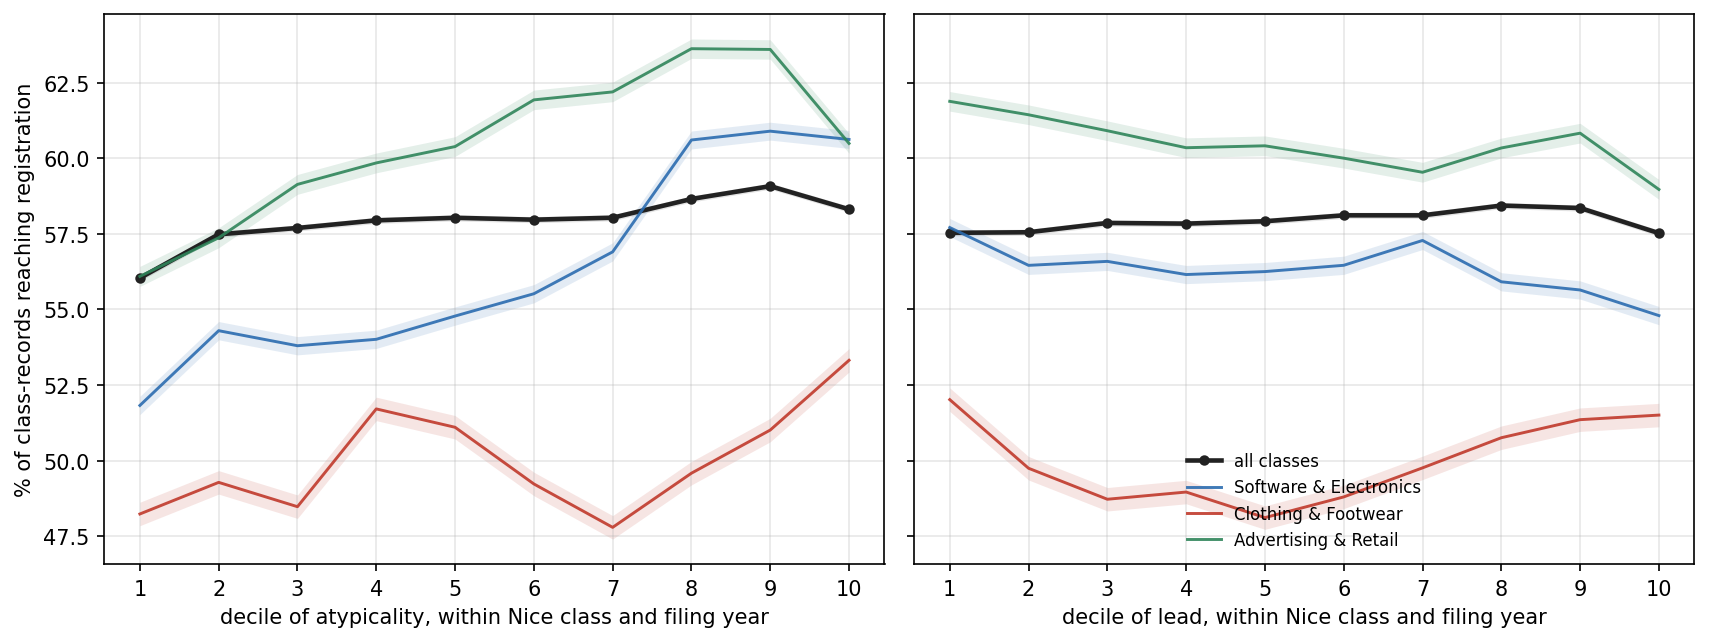
\includegraphics[width=\textwidth]{results/fig_registration_deciles.png}
\caption{Share of class-records reaching registration, filings 1995--2018,
by decile of atypicality (left) and of lead (right), deciles cut within
Nice class and filing year; $n = 9{,}024{,}532$ scored class-records. The
black line pools all 45 classes; the colored lines are three named classes.
The grey band is a 95\% binomial interval on the pooled line.}
\label{fig:regdeciles}
\end{figure}

The flatness of lead at this step has a mechanical reading worth stating:
lead is computed from the five years of filings \emph{after} the filing
date, which had not happened when the examiner acted. No participant in
prosecution could observe the quantity. Whatever small association appears
must run through correlates that were visible at the time --- the words
themselves, the industry, the drafter. Atypicality's past-facing half, by
contrast, is exactly what an examiner steeped in the class's usual language
experiences, and it is the axis registration responds to.

Figure~\ref{fig:regplane} shows the same outcome on the two surprise axes
directly, for the two largest classes: each hexagonal cell is colored by
the share of its filings that registered. The color gradient runs along
the diagonal --- from the low-surprise corner, where registration is
lowest, up through the middle of the range --- and barely across it.
Distance from the diagonal is lead; position along it is atypicality. The
plane says graphically what the deciles say numerically: the examination
step reads how far a filing sits from its class's usual language, not
which direction it faces in time.

\begin{figure}[!htbp]\centering
\includegraphics[width=\textwidth]{results/fig_registration_plane.png}
\caption{Share reaching registration across the surprise plane, filings
1995--2018 in the two largest classes. Each hexagon holds at least 50
class-records and is colored by the share of them that registered; the
dashed line is $K^- = K^+$, on which lead is zero. Cells below the line
are leading, cells above lagging.}
\label{fig:regplane}
\end{figure}

Two cautions on reading the level. First, registration is mostly a measure
of the applicant's own follow-through: of the applications that do not
register, roughly nine in ten die by inaction --- the applicant never
files the statement of use, or stops responding during prosecution --- and
only 4.3\% are removed adversarially (Table~\ref{tab:funnel}). Second,
the shape depends on how the deciles are cut. If the deciles are instead
cut on the pooled distribution, and the sample restricted to debut
filings, the atypicality curve becomes an inverse-U with a deeper
conventional tail: 46.6\% at the bottom, about 58\% in the middle,
53.4\% at the top. That version mixes in class and cohort composition; the supplementary
material reports it, with the reasons familiarity alone cannot produce
the shape. The within-cell profile of
Figure~\ref{fig:regdeciles} is the cleaner statement, and on it the
conventional tail, not the atypical one, is the penalized end. The shape
is the one audience-conformity research predicts for evaluators
\citep{Zuckerman1999, Hsu2006, Zhao2017}, here from an examiner and at
census scale; \citet{TaeuscherRothe2020} find settings where the optimum
sits off-centre.

\subsection{Examination rewards a middling specificity}\label{app:registration}

Across 3.59 million debut filings (57.6\% base rate), completion is an
inverse-U in \emph{atypicality}: it climbs from 46.6\% at the least atypical
end to about 58\% in the middle and falls back to 53.4\% at the most atypical
(Figure~\ref{fig:profiles}, panel C). The same shape appears on the
past-facing level alone, more mildly, running 54.0\% at the bottom quintile to
58.4--59.1\% in the middle and 57.7\% at the top (Figure~\ref{fig:outcomes}A).

The signed axis behaves differently. Completion on $L$ falls to a trough of
51.9\% just above the median and then rises steadily to 58.0\% at the leading
end. That trough is composition rather than timing. Lead magnitude
correlates with atypicality at $+0.31$, so the filings near zero lead are
disproportionately the low-atypicality filings, and those complete poorly
for the reason above. Splitting by atypicality confirms it: the trough is
absent in the upper three fifths and survives only in the lowest. The
signed axis still enters a linear specification strongly
(harmonized estimates in the companion paper), but monotonically rather than through an interior
peak: what curvature exists at registration belongs to how far a filing's
language sits from its category, not to which side of it the filing sat.

\begin{figure}[!htbp]\centering
\includegraphics[width=\textwidth]{results/debut_outcome_topic.png}
\caption{Outcomes for debut filings (owner's first-ever filing) across all
45 Nice classes under theme scoring, filing years 1995--2018, in quantile
bins with 95\% intervals, quantiles cut on the pooled distribution.
$n = 3{,}589{,}068$; registered subset $n = 2{,}066{,}600$. \emph{A:}
P(reached registration). \emph{B:} P(owner ever in SEC EDGAR, the
Commission's public filing system $\mid$ registration).}
\label{fig:outcomes}
\end{figure}

\begin{figure}[!htbp]\centering
\includegraphics[width=\textwidth]{results/quintile_profiles.png}
\caption{Quintile profiles for the three outcomes. \emph{A:} the share of
registrations failing the five-year proof of continued use, by lead
quintile, adjusted within Nice class and registration year with the
drafting and filer controls of Table~\ref{tab:gate_lpm}; the dashed line
is the rate for all registrations. The profile rises gently and
monotonically through the fourth quintile and then steps up: about seven
tenths of the top-to-bottom gap is the single step from the fourth
quintile to the fifth, seven times the average step below it. \emph{B:}
the share of first-time filers whose owner ever reaches SEC reporting, by
quintile of atypicality and of lead, adjusted within Nice class and filing
year with description length held. \emph{C:} raw registration rates for
debut filings in twenty bins, cut on the pooled distribution --- an
inverse-U on atypicality, and on lead a trough just above the median that
is compositional, absent once atypicality is held in its middle fifth
(dashed). Horizontal line at the pooled rate.}
\label{fig:profiles}
\end{figure}

\begin{figure}[!htbp]\centering
\includegraphics[width=0.9\textwidth]{results/fig_registration_sankey.png}
\caption{The registration step as a flow, unique serials filed 1995--2018
($n = 6{,}877{,}795$), split by counsel of record on the filing.
Represented applications reach registration at 61.9\%, self-filed at
45.6\%.}
\label{fig:sankey}
\end{figure}

The obvious objection is that unfamiliar language is simply refused more
often, so the measure recovers nothing beyond familiarity. Completion falls at
\emph{both} ends, so the most category-typical filings also complete less than
the middle, which familiarity cannot explain; and the curvature is specific to
the unsigned axis, the signed axis showing no interior peak at all.

Refiling after abandonment is itself mildly related to vocabulary position,
though not on the axis that matters here. Refiling rates are flat in
atypicality (a middle-minus-tails difference of $-0.06$pp on a 3.6\% base) but
rise with lead, from 2.6\% among the most lagging abandoned applications to
3.4\% among the most leading.


\input{gen_val_gate}
\subsection{The construct is not patenting}\label{sec:patent}

Within the firms that do both, trademark vocabulary and patenting move
independently. On a panel of trademark owners name-matched to PatentsView
patent assignees \citep{PatentsView}, each axis is regressed on
$\log(1 + \mathrm{patents})$ with firms absorbed and errors clustered on
the firm, estimated on 94{,}181 firm-years across 17{,}506 firms under
theme scoring (93{,}551 and 17{,}415 under term scoring) --- 134{,}075
matched firm-years before dropping the firm-years that contribute no
within-firm variation. The outcome is standardized, so $\beta$ is the
shift in standard deviations of the axis per unit of log-patents; one
unit is roughly a tripling of the patent count, and a firm going from
none to twenty moves about three units.

\begin{center}\small
\begin{tabular}{llrrr}
\toprule
Text counted as & Axis & $\beta$ (sd) & $t$ & Between-firm $r$ \\
\midrule
Themes & atypicality & $+0.012$ & $+3.0$ & --- \\
Themes & lead        & $-0.058$ & $-9.4$ & $-0.020$ \\
Terms  & atypicality & $-0.055$ & $-11.5$ & --- \\
Terms  & lead        & $+0.012$ & $+2.0$ & --- \\
\bottomrule
\end{tabular}
\end{center}

\noindent The grid is close to a mirror: whichever axis carries the small
signal under one way of counting the text carries the opposite sign under
the other. The theme-scored \emph{lead} coefficient ($-0.058$) and the
term-scored \emph{atypicality} coefficient ($-0.055$) are nearly the same
number attached to different quantities. Only those two cells are
established; the mirror's other diagonal is within noise, and the
orthogonality conclusion rests on the magnitude bound --- every cell
under $0.06$ standard deviations --- rather than on any cell's sign.
Nothing here reaches a tenth of a standard deviation.

One objection is timing: a patent is applied for before its invention is
in public use and a trademark when the firm is ready to sell, so patents
would lead. Firms do not proceed that linearly \citep{Seip2018}, and no
timing offset from $t-2$ to $t+1$ isolates a direction ($-0.054$ to
$-0.089$ sd under theme scoring, $+0.012$ to $+0.024$ under terms);
among owners who both patent and raise a priced round, neither event
systematically precedes the other (median lag zero years).

The second objection is heterogeneity: a pooled near-zero could hide a
positive slope where the two rights are complements offsetting a negative
one where trademarks work alone. On a coarse, judgement-based sorting of
classes into complements and substitutes --- assigned in advance from the
class definitions, nothing estimated --- the slopes are $-0.000$ among
complements, $-0.026$ among substitutes, interaction $-0.008$
($t = -0.49$), and the complement classes do not agree in sign with one
another (cell detail in the supplementary material). Neither retention
supports the complementarity story, with the caveats that a coarse
sorting can miss a finer-grained one and that conditioning on a
successful assignee match pushes any interaction toward zero.


\subsection{SEC reporting: the lead profile survives the design; the atypicality gradient is composition}\label{sec:bluesea}

The outcome here is the firm-level one that the representation hazard
of Section~\ref{sec:hazard} turns on: whether an owner ever appears in the Securities and
Exchange Commission's financial reporting records. That is broader than
exchange-listed: roughly half the matched firms carry a ticker and the
rest report for other reasons. Figure~\ref{fig:successcurves} draws the
raw rate against each axis in twenty bins. In signed lead the profile is a
U whose tails both sit above the base rate and whose lagging tail is the
higher; in lead magnitude and in atypicality the raw rate rises.

\begin{figure}[h]\centering
\includegraphics[width=\textwidth]{results/fig_success_ventiles.png}
\caption{Share of registered debut owners (first registered filing
1995--2018, $n = 2{,}066{,}600$) ever appearing in SEC EDGAR, in twenty
equal-count bins of debut lead $L$, lead magnitude $|L|$, and atypicality
$A$, cut on the pooled distribution. Bands are 95\% binomial intervals;
the dashed line is the 0.65\% base rate. These are raw rates carrying
class, year and length composition; Table~\ref{tab:edgar} gives the
design-based estimates, under which the atypicality gradient is absorbed
and the signed-lead U remains.}
\label{fig:successcurves}
\end{figure}

The raw atypicality gradient does not survive the design-based estimates
(Table~\ref{tab:edgar}). Within class and filing year, holding description
length fixed, top-quintile atypicality raises the probability of SEC
reporting by $+0.000$pp on a 0.481\% base ($t = 0.0$), and by $-0.003$pp
on the past level alone. The quintile profile is not even monotone: the
three middle quintiles sit \emph{below} the bottom one and the top merely
returns to it. The 2.7-fold gradient in the raw bins is composition:
firms that go on to report cluster in particular classes, years, and
multi-class filings, and class$\times$year fixed effects absorb it. Lead
costs, at equal atypicality: the signed component enters negatively
($-0.047$pp per standard deviation, $t = -7.8$) while the unsigned
component enters positively ($+0.067$pp per standard deviation,
$t = 7.7$). The U in the raw bins is exactly this pair: lagging filings
show the magnitude premium with no lead penalty, leading filings show it
net of that penalty, and the middle bins show neither. Once the levels
are controlled, the recovery of the far-leading tail is much reduced: the
quintile profile falls through Q4 and recovers only slightly at Q5.

\begin{table}[h]\centering\small
\caption{Debut listing and vocabulary position: design-based estimates.
LPM of P(owner ever in SEC EDGAR) on 1{,}556{,}968 registered debut
filings 1995--2018, one observation per owner, class$\times$filing-year
fixed effects, heteroskedasticity-robust SEs. Quintiles cut within
class$\times$year. Base rate 0.481\%.}
\label{tab:edgar}
\begin{tabular}{lrr}
\toprule
 & Coefficient (pp) & SE \\
\midrule
\multicolumn{3}{l}{\emph{Atypicality quintiles, $A = \tfrac{1}{2}(K^{-}+K^{+})$ (Q1 omitted)}} \\
\quad Q5, FE only & $+0.017$ & $0.018$ \\
\quad Q5, FE + log length & $+0.000$ & $0.018$ \\
\quad Q5, FE + log length, on $K^{-}$ alone & $-0.003$ & $0.018$ \\
\midrule
\multicolumn{3}{l}{\emph{Signed lead quintiles, FE + log length + KL levels}} \\
\quad Q3 & $-0.133$ & $0.020$ \\
\quad Q4 & $-0.187$ & $0.021$ \\
\quad Q5 & $-0.158$ & $0.024$ \\
\midrule
\multicolumn{3}{l}{\emph{Decomposition, FE + log length}} \\
\quad lead magnitude $|L|$ (pp per sd) & $+0.067$ & $0.009$ \\
\quad signed lead $L$ (pp per sd) & $-0.047$ & $0.006$ \\
\quad log description length & $+0.056$ & $0.004$ \\
\bottomrule
\end{tabular}
\\[0.3em]\footnotesize Standard errors in place of significance stars; see
the note to Table~\ref{tab:gate_lpm}.
\end{table}

Owners are matched to SEC registrants by normalized exact name, over a
candidate universe of all 5.67 million owners in the corpus; names
resolving to more than one registrant are dropped rather than assigned,
and one match is kept per owner string. That yields 19{,}889 matched
owners covering 7{,}588 registrants, and a base rate of 0.481\% among
registered debut filers. Validation on 22 companies that indisputably went
public --- across software, pharmaceuticals, food, apparel, aerospace and
autos --- matches all 22. A random sample of 25 matches carrying at least
three filings was inspected by hand and none was wrong, which is a check
on gross failure modes rather than a precision estimate.

The linkage is nonetheless a name match, and that bounds the atypicality
reading in particular. Firms with distinctive names are easier to match
than firms with generic ones, and distinctiveness of a name plausibly
travels with distinctiveness of the goods/services text; nothing in this
design separates the two. The lead coefficient is unchanged under
alternative linkages; the atypicality coefficient is not, so only the
lead result is robust to the name-match design.

The U is also not atypicality working through lead's construction (the
mechanical coupling stated in Section~\ref{sec:three_scorings}): on this
sample lead magnitude and atypicality correlate at $+0.25$, signed lead at
only $-0.10$, and cutting lead fifths within fifths of atypicality keeps
the structure: the most lagging fifth out-reports the most leading in four
of the five atypicality strata (by $0.08$ to $0.39$pp on sub-1\% bases),
and the ordering reverses only in the most atypical fifth, where the most
leading debuts report most. The lagging tail's premium is not a ceiling
artifact; the leading tail's partial recovery in the raw U is where the
atypicality composition lives, which is what the level controls in
Table~\ref{tab:edgar} absorb.

``SEC reporting'' is not ``went public'': splitting matched owners on
whether their SEC filer number carries a ticker gives $10{,}556$ listed
against $9{,}333$ reporting without one, and both halves show the same U
in lead (Section~\ref{sec:robust}), so the result is not an artifact of
counting non-operating registrants as successes.


\subsection{Firm-level outcomes depend on the representation}\label{sec:hazard}

The mark-level results above hold under theme and term scoring alike.
The firm-level results do not, and the divergence is the second hazard
this paper documents. Under term scoring, leading filings appear to belong
to better firms; under theme scoring, on identical samples, every signed
version of that finding dissolves or reverses. What follows reports the
term-scored results as they would be published, then what happens to each
under distribution scoring, and then why.

\label{sec:robust_hazard}

Under term-level scoring, leading filings appear to belong to better
firms, and the appearance is consistent across three outcomes. Among
registered debut filings, the probability that the owner ever appears in
SEC EDGAR rises in term-\dkl{} from 0.29\% at the bottom quintile to
0.42\% at the top. On an SEC-matched firm-year panel, a firm's trailing
3-year mean term-\dkl{} predicts its gross margin at $+2.2$pp per
standard deviation ($t = 2.7$ on the locally rebuilt panel through 2019;
$+3.2$pp, $t = 5.3$, on the published panel through 2024), with
past-facing surprise entering positively and future-facing negatively.
And firm-year term-\dkl{} predicts excess stock returns of $+1.5$ to
$+5.0$pp per standard deviation at one-to-four-year horizons. (A larger
debut-only return figure, $+28$pp at 4 years, fails a sample-size
diagnostic and is not claimed.)

None of these signed results survives when the same text is scored on
themes instead of words. On identical samples, the debut listing
gradient in signed theme-\dkl{} is flat to declining. The margin
coefficient reverses sign --- $-1.3$pp per standard deviation
($t = -1.8$) at $T = 50$, $-2.2$pp ($t = -3.1$) at $T = 200$, and
$-0.8$pp ($t = -1.1$) at $T = 500$, against the term-level $+2.3$pp ---
and the past-/future-facing decomposition flips sign and stays flipped.
The term-level listing gradient separately dissolves under
document-length controls: within bands of equal length it is U-shaped
rather than rising, and the monotone rise is contributed by composition
across lengths, because listed firms' counsel write longer descriptions.
The mark-level results, by contrast, are unaffected --- they hold under
both scorings at every resolution.

One rescue for the signed signal must be ruled out. The theme model's
vocabulary is built from a sample, so rare and emergent terms are
invisible to it; if the firm signal lived exactly in those terms, theme
scoring would be erasing a real signal rather than an artifact. To test
this, each filing's share of vocabulary invisible to the theme model is
computed --- 63.8\% of the software class's term \emph{types}, though
only about 9\% of its token \emph{mass}. That share is itself a strong
firm marker: P(EDGAR) runs from 2.9\% to 5.5\% across its quintiles, and
survival at the five-year proof improves by $+5.7$pp. But \emph{within}
strata of equal invisible share, the signed \dkl{} gradient on the firm
outcome is flat to negative, while the mark-level penalty holds in both
strata ($-6.9$ and $-8.3$pp). The firm-level signal that term scoring
finds is unsigned specificity: serious firms describe specific products
with specific, therefore rare, words, and rare-term mass inflates
term-\dkl{} mechanically. Note that raising the theme count does not
test this --- a crypto/blockchain theme exists at $T = 200$ but not at
$T = 50$ or $T = 500$, because raising $T$ re-partitions the same fixed
vocabulary rather than extending it --- so resolution sweeps test
granularity, not coverage, and the invisible-share split is the test
that settles the question.

The registration filter does not explain the divergence either. Dropping
the registration conditioning leaves the term-level listing gradient
essentially unchanged (0.26\% to 0.38\% across quintiles against 0.29\%
to 0.42\% conditional), and an examiner channel touching 4.3\% of failed
applications cannot generate several-point quintile gaps.

The hazard, stated for reuse: term-resolved text-novelty measures can
manufacture firm-performance correlations out of drafting style and
lexical specificity, and a distribution-based rescoring --- one model
fit --- is a cheap, decisive diagnostic.

\section{Robustness: what changes under other choices}\label{sec:robust}

Each result in Section~\ref{sec:validation} is stated under one formulation chosen for legibility: one
theme resolution, flat weighting inside the reference windows, symmetric
five-year windows, estimates conditional on grant, and the 2002--2018
registration cohorts. This section reports what each of those choices costs,
and in each case states the more complicated finding beside the simpler one
the body uses.

\subsection{Representation and weighting}

A scoring is fixed by two choices. The \emph{representation} is what the
language is turned into: a distribution over 50 fitted themes, or a
distribution over the class vocabulary's terms. The \emph{weighting} is
how days inside the reference window count: every day equal, or decaying
by half every two years. Every reference is per-filing, anchored on the
filing's own date (Section~\ref{sec:construct}). Four builds exist:

\begin{center}\small
\begin{tabular}{llrr}
\toprule
Representation & Weighting & sd(lead) & sd(atypicality) \\
\midrule
Themes & flat          & $0.102$ & $0.698$ \\
Themes & half-life 2y  & $0.082$ & $0.698$ \\
Terms  & flat          & $0.155$ & $1.101$ \\
Terms  & half-life 2y  & $0.130$ & $1.102$ \\
\bottomrule
\end{tabular}
\end{center}

\noindent All four are compared on the 6.01 million filings every one of
them scored. The first row is the production scoring.

Changing one choice at a time settles the ordering. Correlations of lead
between builds differing in exactly one respect:

\begin{center}\small
\begin{tabular}{lrr}
\toprule
Choice varied & $r$ (lead) & $r$ (atypicality) \\
\midrule
Weighting, flat vs half-life 2y (themes)  & $0.982$ & $1.000$ \\
Weighting, flat vs half-life 2y (terms)   & $0.970$ & $1.000$ \\
Resolution, 50 vs 200 themes\footnotemark              & $0.636$ & $0.828$ \\
Representation, themes vs terms           & $0.460$ & $0.396$ \\
\bottomrule
\end{tabular}
\end{center}

\footnotetext{The resolution row is computed on the five-year-proof sample
rather than the 6.01 million-filing common sample of the other rows.}
\noindent The weighting is close to irrelevant: whether recent language counts
for more than distant language within the window barely moves the score, and it
does not move atypicality at all to three decimals, which is what the
$45$-degree rotation of Section~\ref{sec:construct} implies --- the long axis is
a property of the filing and the weighting acts almost entirely on the small
residual. Resolution and representation matter
most: quadrupling the number of themes leaves the two builds agreeing on 40\%
of the variance in lead, and themes against terms on less than a quarter. A
robustness check that varies only the weighting is therefore close to a
restatement; one that varies the representation or the resolution is a real
test, which is why the term-scored replication in Appendix~\ref{app:scoring}
and the sweep below are the ones the claims lean on.

\subsection{Theme resolution}

Fifty themes over a 62,168-term vocabulary is roughly one theme per
industry; whether the findings depend on that coarseness is testable by
refitting at higher $T$. Raising the theme count does not add coverage --- the
vocabulary is fixed, and a larger $T$ re-partitions the same words --- but it
changes what counts as sitting far from an industry, and could change any sign.
Re-fitting the model at four resolutions on the same stratified sample and the
same analyzer, and re-scoring the software class under per-filing windows:

\begin{center}\small
\begin{tabular}{rrrrr}
\toprule
Themes & Proof contrast, lead & $t$ & Proof contrast, atypicality & $r$ with $T=50$ \\
\midrule
$50$   & $+3.23$pp & $13.8$ & $-14.01$pp & --- \\
$100$  & $+2.71$pp & $11.6$ & $-13.69$pp & $0.690$ \\
$200$  & $+5.20$pp & $22.2$ & $-13.45$pp & $0.640$ \\
$500$  & $+5.69$pp & $24.3$ & $-14.49$pp & $0.641$ \\
\bottomrule
\end{tabular}
\end{center}

\noindent Three readings, in descending order of how much weight they carry.
The sign and the significance are untouched across a tenfold change in
resolution, and so is atypicality, which stays within a point of $-14$pp
throughout. The magnitude is not: it does not move monotonically in $T$, so
no single resolution can be quoted as the software class's effect, and the
figure this paper reports at
$T = 50$ sits at the low end of the range rather than the high one. A fifth
fit at $T = 1000$ exists and is excluded: its first run shipped
undertrained models through an indentation bug, and the refit is not
persisted. And
agreement with $T = 50$ settles at $0.64$ without decaying as $T$ grows, which
says the resolutions share a fixed core and differ in the remainder rather than
drifting apart as the partition refines.

The corpus-wide contrast is steadier than the single class: at $T = 200$,
scored for all 45 classes, it is $+2.23$pp against $+2.29$pp at $T = 50$. Only
those two resolutions exist corpus-wide, so that is a two-point comparison, but
it is the one the paper's estimates run on, and pooling evidently averages away
much of the per-class resolution sensitivity.

\subsection{Fitting noise at one resolution}

The sweep leaves one question open. Scores at different resolutions agree at
$r = 0.64$ to $0.69$ on lead, and neighbouring resolutions agree no better than
distant ones. That has two readings. The number of themes may genuinely change
what is being measured. Or a theme-model fit may be unstable, with two runs settling in different
local optima, in which case the sweep measures
fitting noise and the resolution has little to do with it.

Holding $T$ fixed and moving only the seed separates the two. A second fit at
$T = 200$ on the same sample, the same vocabulary and the same number of
passes, differing from the first in nothing but its random seed, agrees with
it at $r = 0.79$ on lead and $r = 0.87$ on atypicality across 1.11 million
scored software-class filings. The cross-resolution figures were $0.64$ and
$0.83$. Most of what the sweep showed as resolution sensitivity is therefore
present between two fits that differ only in the seed: for atypicality nearly
all of it, for lead well over half. The resolutions are not measuring
different things; each fit is a noisy draw on the same thing.

The estimate moves less than the scores do. On the identical sample, the
five-year-proof lead contrast is $+5.20$pp under the first seed and $+4.88$pp under
the second (SE $0.23$ each), and the atypicality contrast $-13.45$ and
$-14.38$pp. Two consequences follow. A single fit's lead score carries
measurement error of roughly a fifth of its variance, which attenuates every
coefficient on lead toward zero; correcting for it would enlarge the
estimates, not shrink them. And the spread of
magnitudes across the resolution table above, which does not move
monotonically in $T$, should be read as a band about a third of a point wide
from fitting noise alone rather than as a property of any particular $T$.

The substantive claim does not depend on any of this. The five-year-proof
lead contrast on the 2002--2018 registrations each build scores runs
$+2.29$, $+1.95$, $+3.56$ and $+2.92$pp across the four builds in the
order tabulated above, and the atypicality contrast $-4.39$, $-4.43$,
$-3.63$ and $-3.73$pp. Every sign holds; term scoring returns the larger
lead contrast, so the headline estimate is the conservative
representation.

\subsection{Decayed reference windows}\label{sec:robust_decay}

Inside the reference windows every day counts the same. The alternative
weights recent language up, with a half-life of two years inside the same
1,826-day truncation, so that a term the class adopted last month is more
familiar than one it adopted four years ago. Rescoring the corpus that way
changes the scores little and the estimate somewhat. Flat and decayed lead
correlate at $0.980$ on the 3.10 million gate registrations and atypicality
at $1.000$ to three decimals. On the identical registrations, with quintiles
cut within class and registration year, the top-minus-bottom gate contrast
on lead is $+2.29$pp under the flat window and $+1.95$pp under the decayed
one (SE $0.09$ each); on atypicality it is $-4.39$ and $-4.43$pp. The
decayed window therefore returns a lead penalty about a seventh smaller,
with the same sign, the same precision, and the same profile. The flat
window is kept in the body because it is the simpler statement; a reader who
prefers recent language to count for more should take $+1.95$pp as the
estimate.

\subsection{Window width}\label{app:wsweep}

The window is a parameter of the measure, not a property of it, and the five
years used throughout was inherited from the class-year construction rather
than chosen under the current one. Re-scoring the software class at several
widths under per-filing references, and judging each by the five-year-proof
quintile contrast it produces, gives $+2.02$pp at two years, $+2.20$ at
three, $+3.23$ at five and $+3.37$ at seven, each on an identical sample of
452{,}911 registrations and each with a standard error of $0.23$pp. Signal
rises steeply from two to five years and is flat between five and seven: the
$+1.03$pp gain from three to five is well outside the sampling error, the
$+0.14$pp from five to seven is not. A ten-year window returns $+2.89$pp,
but that figure is not comparable to the others --- requiring both windows
to lie inside the corpus costs 22\% of the scored filings and 13\% of the
gate sample, dropping the earliest and latest registration years, which are
also the years whose contrasts differ most. The apparent decline at ten
cannot be separated from that change in composition and is not evidence
about window width. On the range where the sample is fixed, seven years is
nominally the peak and five is within noise of it while retaining more of
the corpus, so five is defensible rather than optimal. The sweep is on one class
and one outcome.

\subsection{Mixing the two windows}\label{app:wmix}

``Leading'' is relative to a reference, and the two references need not be
the same width. A short past and a long future make lead a measure of
foresight --- whether the filing resembles where the class was heading over
the next seven years more than what it wrote in the last three. A long past
and a short future make it a measure of rupture --- whether the filing has
broken with what the class had established over seven years, judged against
only the next three. Scoring every class on the production representation
and per-filing windows at $W \in \{3, 5, 7\}$ years on each side, and
evaluating all five variants on identical samples --- the gate columns on
the 3.10 million registrations 2002--2018, quintiles within
class$\times$registration-year; the registration columns on the scored
filings 1995--2018, quintiles within class$\times$filing-year:

\begin{center}\small
\begin{tabular}{llrrrr}
\toprule
Variant & Past, future & \multicolumn{2}{c}{First-gate failure} & \multicolumn{2}{c}{Registration} \\
 & (years) & Q5$-$Q1 (pp) & classes $>0$ & Q5$-$Q1 (pp) & Q3 $-$ tails \\
\midrule
Foresight     & 3, 7 & $+1.65$ (0.09) & 31 of 45 & $+1.09$ & $+0.50$ \\
Symmetric     & 3, 3 & $+1.69$ (0.09) & ---      & $+0.79$ & $+0.13$ \\
Symmetric     & 5, 5 & $+2.29$ (0.09) & 33 of 45 & $+0.71$ & $+0.28$ \\
Symmetric     & 7, 7 & $+2.58$ (0.09) & ---      & $+0.48$ & $+0.65$ \\
Past-rupture  & 7, 3 & $+3.00$ (0.09) & 37 of 45 & $+0.01$ & $+0.33$ \\
\bottomrule
\end{tabular}
\end{center}

\noindent The symmetric five-year row is the paper's FE-only estimate in
Table~\ref{tab:gate_lpm}, reproduced here to the decimal, which fixes the
scale. The penalty rises monotonically along the mix, from $+1.65$pp under
foresight to $+3.00$pp under rupture, and rupture is the more pervasive
variant, positive in 37 of 44 classes against 31. In software the two are
$+1.82$ and $+5.07$pp. So the use requirement punishes distance from the
class's established language more than it punishes resemblance to its
coming language; but foresight carries a penalty of its own, more than half
the symmetric one, and the separation is a matter of degree rather than
kind.

Registration is a different matter. On the signed axis the top-to-bottom
contrast is at most a point on a 57\% base and the interior-minus-tails
depth at most two thirds of a point, under every mix. The examiner's
response to lead, on this scoring, is close to nil.

\subsection{Without conditioning on grant}\label{sec:robust_uncond}

Figure~\ref{fig:uncond} repeats the lifecycle outcome analysis without the
registration conditioning, on filings 2013--2015 pooled across all classes
(a window whose registrations land by $\sim$2017 and face at least one
Section~8 gate by the 2025 snapshot; the earliest registrations in the
window also face their year-ten renewal, so panel B mixes one and two
gates). Panel A is the unconditional composite, the probability that a
filing both registers and passes the gate, measured over all filings
including the never-registered. It is nearly flat in \dkl{} because two
opposed gradients cancel: registration rises in lead
($61.3$\% to $63.2$\%) while gate survival falls ($44.2$\% to $40.8$\%);
the caption carries the quintile figures.
Conditioning on grant is what separates them. Panel B shows the conditional
gate outcome on the same filings, and it is U-shaped rather than inverse-U
(depth $-2.11$pp), with a clearly penalised leading tail consistent with the
cleaner single-gate cohort of Figure~\ref{fig:s8pooled}.

\begin{figure}[h]\centering
\includegraphics[width=\textwidth]{results/appendix_unconditional.png}
\caption{Filings 2013--2015 pooled across classes, theme-scored on
per-filing reference windows ($n = 1{,}419{,}678$; gated subset
$n = 763{,}902$). \emph{A:} the unconditional composite P(registered and
passed the five-year proof) over all filings. \emph{B:} P(passed $\mid$ registered
and gated) on the same filings. The unconditional view is nearly flat in
lead (22.4\% to 22.1\% across quintiles); conditioning on grant is what
exposes the gradient.}
\label{fig:uncond}
\end{figure}

\subsection{Toggled filters, windows and parameters}\label{sec:robust_matrix}

Each analysis in this paper and in the companion paper was rerun under its
natural parameter toggles, on the identical data. Nothing
reverses a headline claim; two auxiliaries move.

\begin{center}\small
\begin{tabular}{lll}
\toprule
Variant & Baseline $\to$ variant & Reading \\
\midrule
Gate window 3.5--9.0 / 4.5--8.0 & lead $+2.29 \to +2.29$ / $+2.28$pp & window immaterial \\
Registration cohorts 2002--09 & $+2.29 \to +0.98$pp & the era swing \\
Registration cohorts 2010--18 & $+2.29 \to +3.11$pp & penalty concentrated late \\
Atypicality, both cohort halves & $-4.39 \to -4.55$ / $-4.28$pp & stable \\
Internet pattern, narrow core & goods web gap $0.0 \to +2.0$pp & divergence holds \\
Convergence arrival 1\% / 4\% & early$\to$late $+4.4\to+1.6$ & $+5.9\to+1.8$ / $+3.8\to+2.3$ \\
Surge doubling 1.5$\times$ / 3$\times$ & in-surge net $+1.3$pp & $+1.2$ / $+0.9$pp \\
Wave entry window 4y / 8y & order flat & flat under both \\
Recombination floor 2 / 10 & net $-2.8$pp & $-1.2$ / $-3.6$pp \\
Pair-lead presence 0.05 & net $+2.3$pp & $+3.1$pp \\
Combination measures, class 035 & 009 values & recomb $-3.8$; pair-lead $-1.4$ \\
Ladder, counsel / self debuts & reporting lead $-0.19$pp & $-0.26$ / $-0.03$pp \\
Ladder, 2009--13 / 2014--18 & reporting atyp.\ $+0.11$pp & $0.00$ / $+0.19$pp \\
Excluding duplicate-text filings & lead $+2.29$; atyp.\ $-4.39$pp & $+3.05$; $-5.68$pp \\
Excluding Manual-scale texts only & same & $+2.64$; $-5.05$pp \\
\bottomrule
\end{tabular}
\end{center}

\noindent Three of these change what a reader should carry. The lead
penalty at the gate belongs to the 2010--2018 cohorts; the 2002--2009 half
carries a third of it, which is the era swing the companion paper documents, seen
from the other side. The ladder's gradients belong to counsel-represented
debuts --- among self-filers the reporting gradient is a null --- and its
atypicality gradient to the 2014--2018 half. And the pair-lead penalty,
$+2.3$pp in the software class under every parameter tried there, is
$-2.1$pp in advertising and retail on the corpus-wide construction, and
pooled across 43 classes is zero raw and $+0.5$pp net of lead and
atypicality, so it is reported as a bound for one class rather than a
general fact. All artifacts are under
\texttt{paper/v3/\_eval/}.

\subsection{Lead is a small residual}

Past-facing and future-facing KL are highly correlated however scored. On the
complete class-009 corpus under the production scoring they correlate at
$r = +0.988$ ($n = 1{,}109{,}643$). The lead $L$ is therefore a small residual
of two large, stable quantities: both levels have a standard deviation near
$0.70$ nats about a mean of $1.46$, while $L$ has a standard deviation of
$0.109$ --- about a sixth of either level's spread. Only $1.2\%$ of the two
levels' combined variance survives into their difference. That is what makes $L$ sensitive to
anything that inflates the levels; under term scoring the dominant such
thing is document length, and Section~\ref{sec:construct} quantifies the
coupling under both representations. The consequence for the lead is
direct: the standard deviation
of $L$ rises $2.2$--$2.5$-fold across deciles of $A$ under term scoring
and $1.5$--$1.8$-fold under theme scoring, so a unit of lead means roughly
the same thing everywhere only in the theme representation.
Appendix~\ref{app:representation} shows this as a length surface over the
two axes. Two qualifications. Theme scoring returns a finite value for about 65\% of
filings, so the two columns are not drawn from the same set; re-estimating the
term-scored correlations on exactly the theme-scored subset barely moves them,
which puts the contrast down to the representation rather than the sample.
And ``flat'' means no
monotone length gradient rather than constant: class 035 under theme
scoring is mildly U-shaped in $A$. The two scorings agree only
moderately per filing (Pearson $0.46$, Spearman $0.42$ on the 6.01 million
filings both score), which gives their agreement on the mark-level
patterns evidential force and their disagreement on the firm-level
patterns diagnostic force (Section~\ref{sec:robust_hazard}). Across
$W \in \{3, 5, 7\}$, 6.9--10.4\% of filings flip sign. Per-filing noise
attenuates at every aggregation used: firm-year means, token pools,
theme prevalence trajectories.

Alignment with expert innovation judgment is at most suggestive. Firms on
BCG/MIT ``most innovative'' lists sit $+0.09$ standard deviations above the panel mean
under term scoring ($p = 0.22$), $+0.14$ under theme scoring
($p = 0.07$), and $+0.08$ at $T = 200$ ($p = 0.20$). The matched
sample is 41 firms, which is too small to carry weight in either
direction, and the paper draws no inference from it. Patent counts remain
uncorrelated with \dkl{} on the same panel (Pearson $+0.010$).

\subsection{Term scoring as a cross-check}\label{app:scoring}

The snapshot cross-check on the single one-gate-elapsed cohort
(registrations 2016--2018, terminal status 710 versus 701--705/800)
agrees with the event-dated estimates and is scoring-robust: $-5.4$pp
survival across quintiles under theme scoring and $-5.7$pp under term
scoring on the identical sample (Figure~\ref{fig:s8pooled}). Under term scoring, gate survival
\emph{rises} in the raw KL level ($+6.5$pp past-facing, $+7.6$pp
future-facing): atypical text survives the use requirement better
while leading text survives it worse --- the same two-axis
separation as Section~\ref{sec:bluesea}, at the mark level.

\begin{figure}[h]\centering
\includegraphics[width=\textwidth]{results/topic_outcomes_all.png}
\caption{The two mark-level outcomes under theme and term scoring on
identical samples, pooled across classes, by within-class lead quintile
(1 most lagging, 5 most leading). \emph{Left:} the share of registrations
2016--2018 that survived the five-year proof of continued use at years five to six,
read from terminal status codes, where the two representations agree
closely. \emph{Right:} registration completion
(filings 1995--2018), where they do not: the inverse-U in the signed axis
is present under term scoring (depth $+0.048$) and absent under theme
scoring (depth $-0.001$). The gate result is scoring-robust; the
registration curvature on this axis is not, and the registration analysis
reports only the unsigned version.}
\label{fig:s8pooled}
\end{figure}

\subsection{Functional form}

\begin{figure}[h]\centering
\includegraphics[width=\textwidth]{results/curve_shapes.png}
\caption{Binned profiles at the three gates, with the linear reading the
paper's contrasts assume and the shape selected by AIC where that is not
linear. Forty equal-count bins; the dotted line marks the fitted vertex. The
bottom row is the case that matters: a linear fit through the
public-reporting profile slopes downward while the data turn up at both tails.}
\label{fig:shapes}
\end{figure}

Four shapes were fitted to each profile by weighted least squares on 40
equal-count bins (Figure~\ref{fig:shapes}): linear, quadratic, an exponential
$a + b e^{cx}$, and a free-vertex symmetric form $a + b e^{c|x - x_0|}$ meant
to catch a U directly. Selection is by AIC.

\begin{center}\small
\begin{tabular}{llrrrl}
\toprule
Outcome & Axis & $R^2$ line & $R^2$ curve & $\Delta$AIC & Shape selected \\
\midrule
Registration & atypicality & 0.38 & 0.92 & 77.1 & curve, peak at $+1.04$ \\
Registration & lead & 0.08 & 0.17 & 1.9 & (quadratic; weak) \\
Use-proof & atypicality & 0.74 & 0.74 & 0.0 & linear \\
Use-proof & lead & 0.44 & 0.55 & 4.3 & V, vertex $-1.50$ \\
SEC reporting & atypicality & 0.74 & 0.84 & 15.2 & curve, peak at $+2.17$ \\
SEC reporting & lead & 0.13 & 0.59 & 26.3 & V, vertex $+0.30$ \\
\quad listed only & lead & 0.19 & 0.46 & 12.2 & V, vertex $+0.41$ \\
\quad reporting, not listed & lead & 0.07 & 0.67 & 37.2 & V, vertex $+0.24$ \\
\bottomrule
\end{tabular}
\end{center}

\noindent The winning form is a free-vertex $a + b\,e^{c|x-x_0|}$. On the
atypicality rows it is a genuine curve, with fitted exponents between $0.5$
and $1.2$ --- a hump that peaks about one standard deviation above mean
atypicality at registration and about two above it at SEC reporting. On every
lead row the exponent collapses to the order of $10^{-4}$, which turns
$e^{c|x-x_0|}$ into $1 + c|x-x_0|$: what wins there is a \emph{V}, linear in
distance from a vertex. A V beating a parabola says the turn is sharper than a
quadratic allows, not that anything is multiplying.

Vertices are in standard deviations of the axis across filings.

The two rows for SEC reporting are the outcome Section~\ref{sec:bluesea} and
Table~\ref{tab:edgar} actually run on; the listed and reporting-only splits
below them show the same shape on each half, which is why the split does not
change the reading.

AIC here is computed on 40 binned means, not on the millions of underlying
filings, so it ranks shapes rather than testing them. The $77$ at registration
and the $12$ to $36$ at the public-reporting gates are decisive; the $1.9$ at
registration on lead and the $4.3$ at the five-year proof are weak, and those
two rows are better read as ``no worse than linear'' than as curvature.

The non-monotone profiles on signed lead decompose into parts of
different symmetry (Figure~\ref{fig:ldecomp}). Each ventile's deviation
of the listing rate from the base is split, by sequential counterfactual
prediction, into the part atypicality composition alone predicts, the
part exact-duplicate text adds, a linear lead tilt, and a residual. The
symmetric U is carried about half by atypicality composition --- the
spread of $L$ rises with $A$, so both tails of the lead axis hold
atypical filings and the middle holds typical ones --- and about half by
a residual that is itself symmetric in $|L|$: the same conditional lead
magnitude effect Table~\ref{tab:edgar} estimates at $+0.067$pp per
standard deviation. Duplicate-text composition adds almost nothing once
atypicality is held, and the linear tilt is an order of magnitude smaller
than either symmetric part ($-0.07$pp per nat). The fitted vertices above
follow from this arithmetic: a symmetric profile plus a negative tilt has
its minimum shifted right of zero, and a survival hump its maximum
shifted left, which is where the fits put them ($+0.24$ to $+0.41$, and
$-0.4$, standard deviations).

Excluding text-duplicate filings strengthens rather than weakens every
headline gradient. Of the five-year-proof sample, 47\% of registrations
share their exact normalized description with at least one other filing;
dropping them raises the lead contrast from $+2.29$ to $+3.05$pp and the
atypicality contrast from $-4.39$ to $-5.68$pp, and dropping only the
Manual-scale texts (clusters of 100 or more identical filings) gives
$+2.64$ and $-5.05$pp. Identical texts carry identical scores and
cluster at the typical end of the axis, so they dilute both gradients;
neither is created by them.

\begin{figure}[h]\centering
\includegraphics[width=\textwidth]{results/fig_L_decomposition.png}
\caption{The signed-lead listing profile taken apart. \emph{Left:} each
ventile's deviation of P(owner ever in SEC EDGAR) from the 0.65\% base,
on 2.07 million registered debuts 1995--2018, split into the part
predicted by atypicality composition alone (50 quantile bins of $A$),
the part added by an exact-duplicate-text indicator, a linear tilt in
$L$ fitted to the remainder, and the residual; bars stack from zero,
dots are the actual deviations with 95\% intervals. \emph{Right:} the
same profile on all filings and on filings whose normalized description
text is unique in their class; the central dip survives, and deepens,
without duplicated text.}
\label{fig:ldecomp}
\end{figure}

\subsection{Listing against reporting}

``Appears in SEC records'' mixes two populations: companies whose shares trade, and entities that file with
the Commission without ever listing --- private issuers, funds, subsidiaries
registering securities. Splitting the 19{,}889 matched owner strings on whether
their CIK carries a ticker in the Commission's own company-ticker file gives
10{,}556 listed against 9{,}333 that file financial statements without one.

It does not change the finding. Among registered debut owners whose debut
filing is scored, $0.310$\% later appear as listed companies and $0.285$\% as
reporting non-listed ones, and both profiles are U-shaped in lead with vertices
at $+0.41$ and $+0.24$ standard deviations. The listed profile is slightly
flatter and noisier, which is what the smaller and more selected outcome
predicts. Whatever the signed axis is picking up at this margin, it is not an
artifact of counting non-operating registrants as commercial successes, and it
is not specific to the act of listing either.\footnote{Two limits on the split.
The ticker file is a current snapshot, so a company that listed in 2003 and was
acquired in 2011 appears in the non-listed tier; the tiers are therefore
``currently listed'' rather than ``ever listed,'' which will misclassify older
successes downward. And the base rates here are computed on the appendix's own
panel, which conditions on the debut filing carrying a score and so is smaller
than the body's sample.}

\subsection{Filings are not independent draws}

Some of them share an exact position
with another filing, and outcomes cluster within owner --- the
within-owner correlation is 0.38 for gate survival pooled and is mechanically
1.0 for public listing, since listing is a property of the owner and a
firm with hundreds of marks contributes hundreds of identical successes.
The regression tables are unaffected, because the gate regressions cluster
on normalized owner and the firm-level specifications carry one
observation per owner. The raw quintile contrasts of
the companion paper --- the era, theme, internet
and surge tables --- are not: their two-sample standard errors ignore the
owner clustering, and their $t$-statistics overstate precision by roughly a
factor of two, which the text of those sections now carries where the
margins are close. Binning filings without the correction likewise
overstates how much structure the corpus contains: on a
positional grid, correcting cell errors for the clustering design effect ---
the factor by which within-owner correlation inflates the variance of a cell
mean --- cuts
apparent excess dispersion by roughly a quarter on the gate outcome and
by half on listing. Displays of the vocabulary plane are descriptive
here for that reason, and the near-zero pooled correlation between $A$ and
$L$ reported in Section~\ref{sec:construct} does not survive cell by cell
within class, so per-cell contrasts should not be read as within-class
effects.


\section{Practices for trademark-text research}\label{sec:practices}

Three practices follow for research that reads trademark text. First,
score distributions, not words. Word-level divergence is dominated by
description length --- on this corpus the correlation with log distinct
terms reaches $-0.68$ --- and firm-level performance correlations built
on it dissolve or reverse under distribution scoring on identical
samples. Any term-level novelty measure should be accompanied by the
theme-level rescoring that costs one model fit. Second, treat the
registered description as a conformed document. Applicants who refile
rewrite toward their class's typical language from both tails, whoever
drafts the second attempt, so samples of registered marks understate the
atypicality applicants first attempted, and estimates on registered text
are estimates on prosecution-filtered language. Studies using description
similarity or breadth inherit this compression. Third, the two components
of surprise are not interchangeable and should not be pooled. Lead is
robust to every partition, weighting, and window tried here;
atypicality's apparent effects can be artifacts of the partition (its
protective effect at the five-year proof belongs to theme importation,
visible only to global models) or of a control (its listing effect
depends on how description length is held). A study that reports
``novelty'' from trademark text without separating the temporal from the
cross-sectional component may attribute to one what belongs to the other.

For users of the classification itself, one caution: internet-bearing
filings in goods classes survive at rates closer to the technology
classes than to their own, so Nice classes used as industry controls do
not partition the internet economy. And for the maintenance data, one
asset: the five-year proof of continued use is a dated, sworn,
product-level survival record covering every registered mark --- an
outcome the indicator literature has largely left unused, observable for
any cohort more than seven years old at no cost beyond parsing the
prosecution history.

\section{Access}\label{sec:access}

Everything described here is public at
\url{https://github.com/ericsilver/tm-vocabulary}. The repository holds
the corpus build (the parser from TRTYRAP case files to dated events, and
the derived event, extras, and dictionary tables), the theme model and
its vocabulary, the per-filing scores under every construction reported
in Section~\ref{sec:robust}, the owner-link tables, every analysis script,
and every generated figure and table in this paper. The pipeline rebuilds
from the public USPTO, SEC and PatentsView sources.

An interactive online appendix at
\url{https://aporia.institute/tm-vocabulary/online-appendix/} lists every
theme with its leading words and its weight in each Nice class, gives
per-class breakouts of every outcome, and includes a viewer of each
class's registrations on the lead/atypicality plane. Researchers who want
the five-year proof as an outcome without the text measure can take the
event-dated cancellation table directly; those who want the measure on a
different corpus can refit the theme model with the scripts provided.

\section*{Acknowledgements}
I thank Simon DeDeo for suggesting that the text be scored on theme
distributions rather than on words, and Carolina Castaldi for comments
on an earlier draft, for orienting me in the trademark-indicator
literature, and for the references behind the nomenclature of
Section~\ref{sec:nomenclature}. Neither has endorsed the present
version, and all errors and judgements are mine.

\section*{Declaration of competing interest}
The author declares no competing interests. The author's current
employment is unrelated to this work, and the views expressed are the
author's alone.

\section*{Funding}
This research received no specific grant from any funding agency in the
public, commercial, or not-for-profit sectors.

\section*{Data availability}
All code and every generated figure and table are public at
\url{https://github.com/ericsilver/tm-vocabulary}; the derived data tables
(dated prosecution events, event-dated outcomes, the theme model, and
per-filing scores) are published as the repository's \texttt{data-v1}
release, and an interactive per-class online appendix is at
\url{https://aporia.institute/tm-vocabulary/online-appendix/}. The
underlying USPTO, SEC, and PatentsView sources are public.

\section*{Declaration of generative AI in the writing process}
This paper was produced in a sustained collaboration with Claude
(Anthropic), which drafted and revised text and analysis code under the
author's direction. Every analysis decision, every number against its
artifact, and all final text were reviewed by the author, who takes full
responsibility for the content.

\input{../../v3_rp/bibliography_rp}
\end{document}
